% A Q&A chapter available in this template can help you when you want to change settings or need examples of how to get what you want.

\documentclass[10pt,letterpaper]{article}
\usepackage{amssymb,amsmath,amsthm,amsfonts}
\usepackage{multicol,multirow}
\usepackage{calc}
\usepackage{ifthen}

% \usepackage[colorlinks=true,citecolor=blue,linkcolor=blue]{hyperref}
\usepackage[
%   showframe,% Seitenlayout anzeigen
  left=2.5cm,
  right=2.2cm,
  top=1cm,
  bottom=1.5cm,
  %includeheadfoot
]{geometry}





\usepackage{array}
\usepackage{graphicx}
% \usepackage{transparent}
\usepackage{siunitx}
\usepackage{listings}
\usepackage{subcaption}
\usepackage{float}

\usepackage{xcolor} 
\usepackage{textcomp}
\usepackage{lipsum}
\usepackage[hidelinks]{hyperref}
\usepackage{gensymb}

\usepackage{tikz}
\usepackage{verbatim}
\tikzstyle{every picture}+=[remember picture]
\tikzstyle{na} = [baseline=-.5ex]


\usetikzlibrary{arrows,shapes,backgrounds}

\def\vo{\SIrange[range-phrase = --,range-units = single]{0(2)}{10}{\volt}}
\def\am{\SIrange[range-phrase = --,range-units = single]{0(4)}{20}{\milli\ampere}}

%  Include code
% \usepackage{bera}% optional: just to have a nice mono-spaced font
%--------------------------------------------------------------
\colorlet{punct}{red!60!black}
\definecolor{background}{HTML}{EEEEEE}
\definecolor{delim}{RGB}{20,105,176}
\colorlet{numb}{magenta!60!black}

\lstdefinelanguage{json}{
    basicstyle=\normalfont\ttfamily,
    numbers=left,
    numberstyle=\scriptsize,
    stepnumber=1,
    numbersep=8pt,
    showstringspaces=false,
    breaklines=true,
    frame=lines,
    backgroundcolor=\color{background},
    literate=
     *{0}{{{\color{numb}0}}}{1}
      {1}{{{\color{numb}1}}}{1}
      {2}{{{\color{numb}2}}}{1}
      {3}{{{\color{numb}3}}}{1}
      {4}{{{\color{numb}4}}}{1}
      {5}{{{\color{numb}5}}}{1}
      {6}{{{\color{numb}6}}}{1}
      {7}{{{\color{numb}7}}}{1}
      {8}{{{\color{numb}8}}}{1}
      {9}{{{\color{numb}9}}}{1}
      {:}{{{\color{punct}{:}}}}{1}
      {,}{{{\color{punct}{,}}}}{1}
      {\{}{{{\color{delim}{\{}}}}{1}
      {\}}{{{\color{delim}{\}}}}}{1}
      {[}{{{\color{delim}{[}}}}{1}
      {]}{{{\color{delim}{]}}}}{1},
}
%--------------------------------------------------------------

\setlength{\parindent}{0em}

\makeatletter
\renewcommand\paragraph{\@startsection{paragraph}{4}{\z@}%
  {-3.25ex\@plus -1ex \@minus -.2ex}%
  {1.5ex \@plus .2ex}%
  {\normalfont\normalsize\bfseries}}
\makeatother

\begin{document}
\footnotesize
%\raggedright

\begin{center}
  {\huge\sffamily\bfseries IoT Gateways} \huge\bfseries \\
\end{center}
% \setlength{\premulticols}{0pt}
% \setlength{\postmulticols}{0pt}
% \setlength{\multicolsep}{1pt}
% \setlength{\columnsep}{1.8em}
% \begin{multicols}{3}

	
	\section{IoT Gateways}
	This Manual describes how to set up the IoT Gateways. There are three different Gateways available:
	
	\begin{itemize}
		\item Analog (\vo, \am)
		\item Digital (Modbus, (BACnet))
		\item Temperature (pt 100 rtd probes with 2,3,4 - wires)
	\end{itemize}
	
	\subsection{Analog Gateway}
	
	\begin{figure} [h]
		\begin{subfigure}{0.49 \textwidth}
			% define source coordinates
			\begin{itemize}
				\item Input source header (SW3) \tikz[na] \coordinate (a-in);
				\item Output source header (SW2) \tikz[na] \coordinate (a-out);
				\item Programming interface \tikz[na] \coordinate (a-iface);
				\item LED \tikz[na] \coordinate (a-led);
				\item Terminal \tikz[na] \coordinate (a-term);
				\item Reset, Config Button \tikz[na] \coordinate (a-rst);
				\end{itemize}
			\end{subfigure}   
			\begin{subfigure}{0.49\textwidth}
			
			
					% Use a background grid to make it easier to find coordinates
					% When the coordinates have been found, remove the 
					% 'show background grid' option. 
					\tikzstyle{background grid}=[draw, black!50,step=.5cm]
					% \begin{tikzpicture}[show background grid]
					\begin{tikzpicture}[]
						\node [inner sep=0pt,above right, opacity= 1] 
						{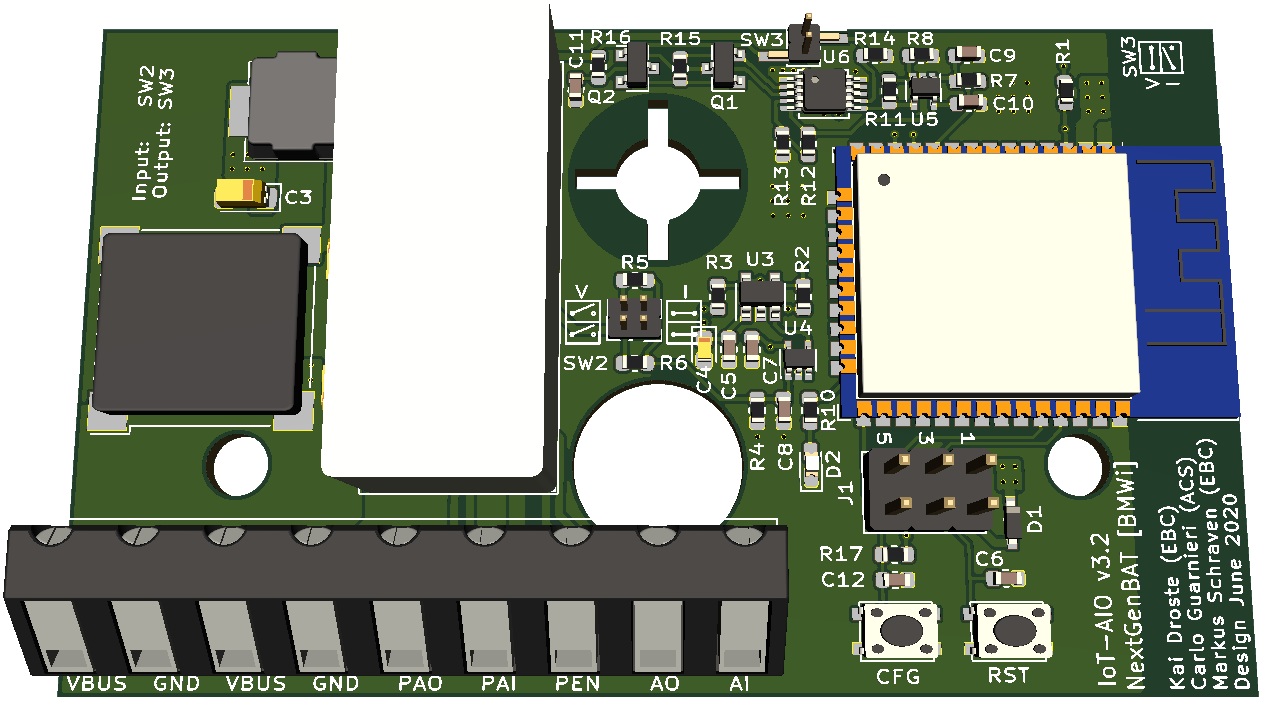
\includegraphics[width=0.95\linewidth]{Figures/analog.png}};
						% show origin
						% \fill (0,0) circle (2pt);
						\draw[red, thick](5.9,0.5) ellipse (0.7 and 0.45);		% Buttons
						\draw[red, thick](3.9, 2.5) circle (0.25); 				%SW2 Input
						\draw[red, thick](5, 4.15) circle (0.25); 				%SW3 Output
						\draw[red, thick](5.8,1.4) ellipse (0.6 and 0.35);		%Programming connector
						\draw[red, thick](0, 0.1) rectangle (4.9,1.2);			%Terminal
						\draw[red, thick](5.02, 1.52) circle (0.18);			%LED
						% define destination coordinates
						\path (5.3,0.2) coordinate (rst)
						(5.5,1.8) coordinate (interface)
						(0,1.0) coordinate (terminal)
						(3.6,2.7) coordinate (SW2)
						(4.8,4.4) coordinate (SW3)
						(4.85,1.6) coordinate (LED);
					\end{tikzpicture}
					
				\end{subfigure}
				\caption{Analog gateway}
				\begin{tikzpicture}[overlay]
					\path[->,black,thick] (a-rst) edge [out=355, in=200] (rst);
					\path[->,black,thick] (a-term) edge [out=0, in=160] (terminal);
					\path[->,black,thick] (a-iface) edge [out=0, in=135] (interface);
					\path[->,black,thick] (a-out) edge [out=0, in=135] (SW2);
					\path[->,black,thick] (a-in) edge [out=0, in=135] (SW3);
					\path[->,black,thick] (a-led) edge [out=0, in=165] (LED);
				\end{tikzpicture}
		\end{figure}
		

		\begin{table}[htpb!]
			\centering
			\caption{Analog terminal}
			\label{tab:a-term}
			\begin{tabular}{lll}
			VBUS 	& + 24 V 	& Input \\
			GND 	& GND 		& Input \\
			VBUS	& + 24		& Output to field device \\
			GND		& GND 		& Output to field device \\
			PAO 	& AO to plc & Not in use \\
			PAI 	& AI to plc & Not in use \\
			PEN 	& + 24 V	& Enable Gateway (necessary) \\
			AO 		& 0 -10 V / 0 - 10 mA & Analog output (single-ended) \\
			AI 		& 0 -10 V / 0 - 10 mA & Analog input (single-ended)\\
	
			\end{tabular}\\ 
		\end{table}

		To set the input to voltage mode, both headers at SW2 need to be disconnected. 
		To set the input to current mode, both headers need to be connected with header jumpers according to the pictogram (I) .\\
		To set the output to voltage mode, the header at SW3 need to be connected with header jumpers according the pictogram (V). 
		To set the output to current mode, the header need to be disconnected.

\newpage
		\subsection{Temperature Gateway}

		\begin{figure} [ht!]
			\begin{subfigure}{0.49 \textwidth}
				% define source coordinates
				\begin{itemize}
					\item Terminal \tikz[na] \coordinate (a-term);
					\item Reset, Config Button \tikz[na] \coordinate (a-rst);
					\item Programming interface \tikz[na] \coordinate (a-iface);
					\item LED \tikz[na] \coordinate (a-led);
					\item Battery tray \tikz[na] \coordinate (a-bat);
					\end{itemize}
			\end{subfigure}
			\begin{subfigure}{0.49\textwidth}
				
				
						% Use a background grid to make it easier to find coordinates
						% When the coordinates have been found, remove the 
						% 'show background grid' option. 
						\tikzstyle{background grid}=[draw, black!50,step=.5cm]
						% \begin{tikzpicture}[show background grid]
						\begin{tikzpicture}[]
							\node [inner sep=0pt,above right, opacity=1] 
							{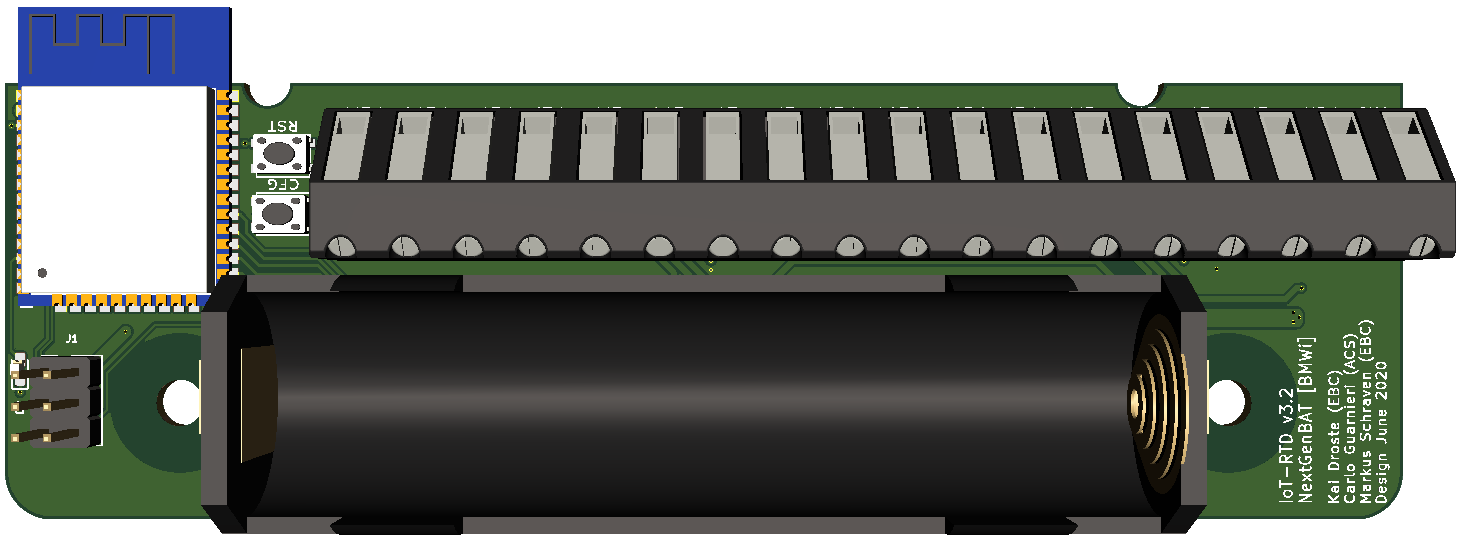
\includegraphics[width=0.95\linewidth]{Figures/temp.png}};
							% show origin
							% \fill (0,0) circle (2pt);
							\draw[red, thick](1.5,1.9) ellipse (0.18 and 0.45);		% Buttons
							\draw[red, thick](0.25,0.75) ellipse (0.25 and 0.4);		%Programming connector
							\draw[red, thick](1.7, 1.5) rectangle (7.9,2.5);		%Terminal
							\draw[red, thick](1, 0) rectangle (6.5,1.4);			%Battery 
							\draw[red, thick](0.05, 0.95) circle (0.14);			%LED
							% define destination coordinates
							\path (1.2,2) coordinate (rst)
							(0.2,1.2) coordinate (interface)
							(2.5,0) coordinate (bat)
							(2.5,2.5) coordinate (terminal)
							(-0.1,0.9) coordinate (LED);
						\end{tikzpicture}
						
			\end{subfigure}
			\caption{Temperature gateway}
					\begin{tikzpicture}[overlay]
						\path[->,black,thick] (a-rst) edge [out=0, in=150] (rst);
						\path[->,black,thick] (a-term) edge [out=10, in=160] (terminal);
						\path[->,black,thick] (a-iface) edge [out=10, in=120] (interface);
						\path[->,black,thick] (a-bat) edge [out=350, in=-170] (bat);
						\path[->,black,thick] (a-led) edge [out=0, in=195] (LED);
					\end{tikzpicture}
			\end{figure}
			
	
			\begin{table}[htpb!]
				\centering
				\caption{Temperature terminal}
				\label{tab:d-term}
				\begin{tabular}{lll}
				GND  	& Do not connect 		& Not in use \\
				PEN 	& Do not connect 		& Not in use \\
				1I-		& 		& RTD probe 1\\
				1V-		& 		& RTD probe 1\\
				1V+ 	&  		& RTD probe 1\\
				1I+		& 		& RTD probe 1\\
				P1I-	& to plc& RTD probe 1 not in use\\
				P1V-	& to plc& RTD probe 1 not in use\\
				P1V+ 	& to plc& RTD probe 1 not in use\\
				P1I+	& to plc& RTD probe 1 not in use\\
				2I-		& 		& RTD probe 2\\
				2V-		& 		& RTD probe 2\\
				2V+ 	&  		& RTD probe 2\\
				2I+		& 		& RTD probe 2\\
				P2I-	& to plc& RTD probe 2 not in use\\
				P2V-	& to plc& RTD probe 2 not in use\\
				P2V+ 	& to plc& RTD probe 2 not in use\\
				P2I+	& to plc& RTD probe 2 not in use\\

		
				\end{tabular}\\ 
			\end{table}

			\paragraph{Set up the gateway for 2,3,4 - Wire RTD-probes}
			In the Configurator pt100 or pt1000 can be chosen. Since the gateways are all setup for pt100 probe, to use pt1000 probes the reference resistor has to be changed on the board (Reference resistor = R13 (or R5), see \autoref{fig:max31865}). \\
		
			To set the gateways for 2, 3 or 4 wires, it is required to solder bridges on the board according to the following image:
			\begin{figure}[ht!]
				
				\begin{minipage}{0.5\textwidth}
					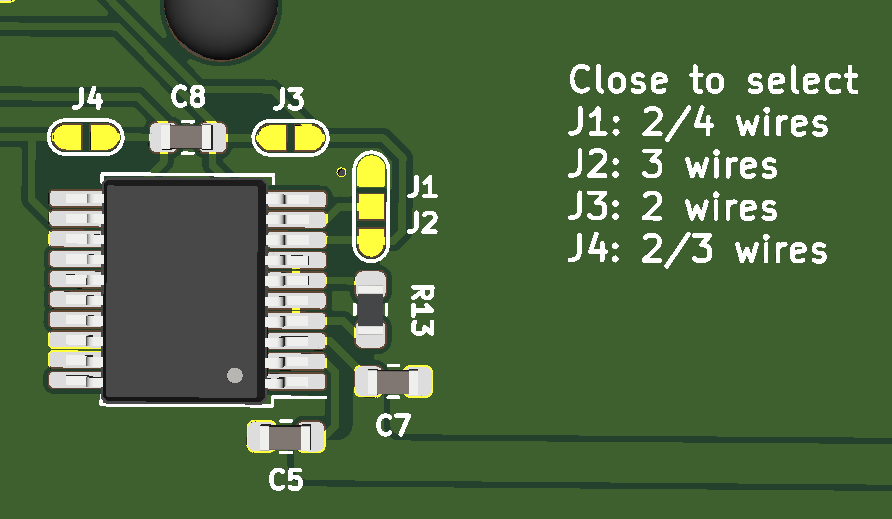
\includegraphics[width=\textwidth]{Figures/rtdsolderpoints.png}
				\end{minipage}
				\begin{minipage}{0.45\textwidth}
					For example: For a three wire probe the solder joints J2 and J4 need to be closed.\\
					% \hspace{1.5cm}
					\begin{itemize}
						\item For a two wire probe, connect V+ and V- with the rtd-probe.
						\item For a three wire probe, connect I+, V+ and V- with the rtd-probe.
						\item For a four wire probe, connect I+, V+, I- and V- with the rtd-probe.
					\end{itemize}

				\end{minipage}
				\caption{Setting the temperature gateway for different types}
				\label{fig:max31865}
			\end{figure}


\newpage
		\subsection{Digital Gateway}

		\begin{figure} [ht!]
		\begin{subfigure}{0.49 \textwidth}
			% define source coordinates
			\begin{itemize}
				\item Programming interface \tikz[na] \coordinate (a-iface);
				\item LED \tikz[na] \coordinate (a-led);
				\item Terminal \tikz[na] \coordinate (a-term);
				\item Reset, Config Button \tikz[na] \coordinate (a-rst);
				\end{itemize}
		\end{subfigure}
		\begin{subfigure}{0.49\textwidth}
			
			
					% Use a background grid to make it easier to find coordinates
					% When the coordinates have been found, remove the 
					% 'show background grid' option. 
					% \tikzstyle{background grid}=[draw, black!50,step=.5cm]
					% \begin{tikzpicture}[show background grid]
					\begin{tikzpicture}[]
						\node [inner sep=0pt,above right, opacity=1] 
						{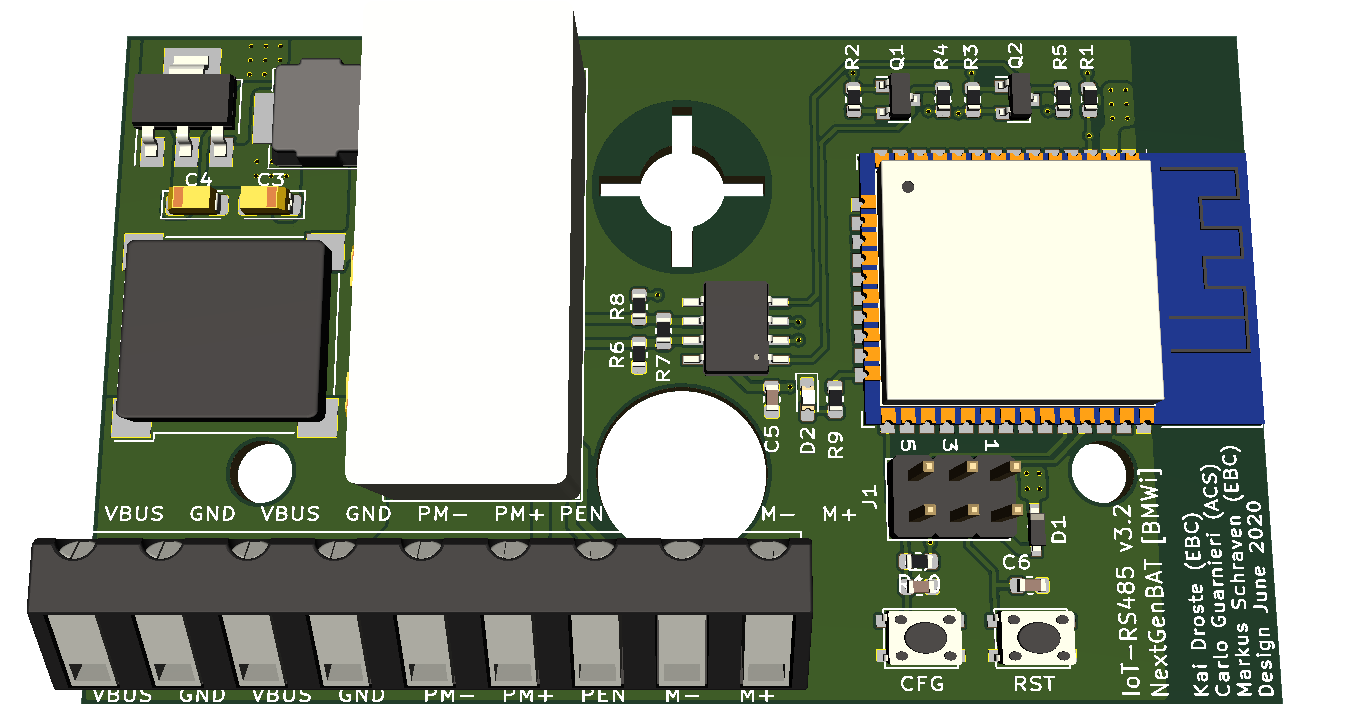
\includegraphics[width=0.95\linewidth]{Figures/digital.png}};
						% show origin
						% \fill (0,0) circle (2pt);
						\draw[red, thick](5.7,0.5) ellipse (0.6 and 0.4);		% Buttons
						\draw[red, thick](5.6,1.3) ellipse (0.5 and 0.3);		%Programming connector
						\draw[red, thick](0, 0.1) rectangle (4.8,1.3);			%Terminal
						\draw[red, thick](4.7, 1.92) circle (0.18);			%LED
						% define destination coordinates
						\path (5.3,0.2) coordinate (rst)
						(5.5,1.6) coordinate (interface)
						(0,1.0) coordinate (terminal)
						(4.5,2.0) coordinate (LED);
					\end{tikzpicture}
					
		\end{subfigure}
		\caption{Digital gateway}
				\begin{tikzpicture}[overlay]
					\path[->,black,thick] (a-rst) edge [out=355, in=210] (rst);
					\path[->,black,thick] (a-term) edge [out=00, in=170] (terminal);
					\path[->,black,thick] (a-iface) edge [out=0, in=110] (interface);
					\path[->,black,thick] (a-led) edge [out=0, in=165] (LED);
				\end{tikzpicture}
		\end{figure}
		

		\begin{table}[htpb!]
			\centering
			\caption{Digital terminal}
			\label{tab:d-term}
			\begin{tabular}{lll}
			VBUS 	& + 24 V 	& Input \\
			GND 	& GND 		& Input \\
			VBUS	& + 24		& Output to field  device \\
			GND		& GND 		& Output to field  device \\
			PM- 	& M- to plc & Not in use \\
			PM+ 	& M+ to plc & Not in use \\
			PEN 	& + 24 V	& Enable Gateway (necessary) \\
			M-		& RS485 - Line &  \\
			M+ 		& RS485 + Line &  \\
	
			\end{tabular}\\ 
		\end{table}

		
% \newpage
	\section{Buttons}
	\label{sec:Buttons}
	The Gateways are equipped with two Buttons.
	The Reset (RST) button restarts the device. The Config (CFG) Button has different functions according to the duration it is pressed.\\
	
	\begin{table}[htpb!]
		\centering
		\caption{CFG Button modes}
		\label{tab:cfg}
		\begin{tabular}{lll}
			Time [sec]					& Function 								& Reaction(LED) \\ \hline
			$t < 1 $				&  \begin{tabular}[c]{@{}l@{}}Eddystone Beacon\\ enable config mode\end{tabular}	& - - 		\\ 
			$1 < t < 3$	&  \begin{tabular}[c]{@{}l@{}}Enable Access Point\\ (works only if not connected to station)\end{tabular}	& ... ... \\ 
			$3 < t < 7$	&  Starts OTA update	& \begin{tabular}[c]{@{}l@{}}Finished: - - - \\ Fail : ...\end{tabular}\\ 
			$t > 7$				& Reset to default settings	& 																 \\ 
			 

		\end{tabular}\\ 
		\begin{flushleft}
			- = Long flash of the LED (1sec)\\ 
			. = Short flash of the LED (\textless 0.5 sec)
			
		\end{flushleft}
	\end{table}

	Since the Gateways support deep sleep mode, it could be necessary to initiate the configuration process with a short press on the RST button. After pressing the RST button, the device needs up to 4 seconds to fully boot up.
\newpage
	\section{Iot Configurator}
	The IoT Configurator is the Webinterface from the IoT-Gateway-Software. 
	It is accessed by redirecting to the IP of the gateway. 
	To find out the right IP of the gateway, the Eddystone-BLE-Beacon (see \autoref{sec:Buttons}) can be used.
	
	\begin{figure}[ht!]
		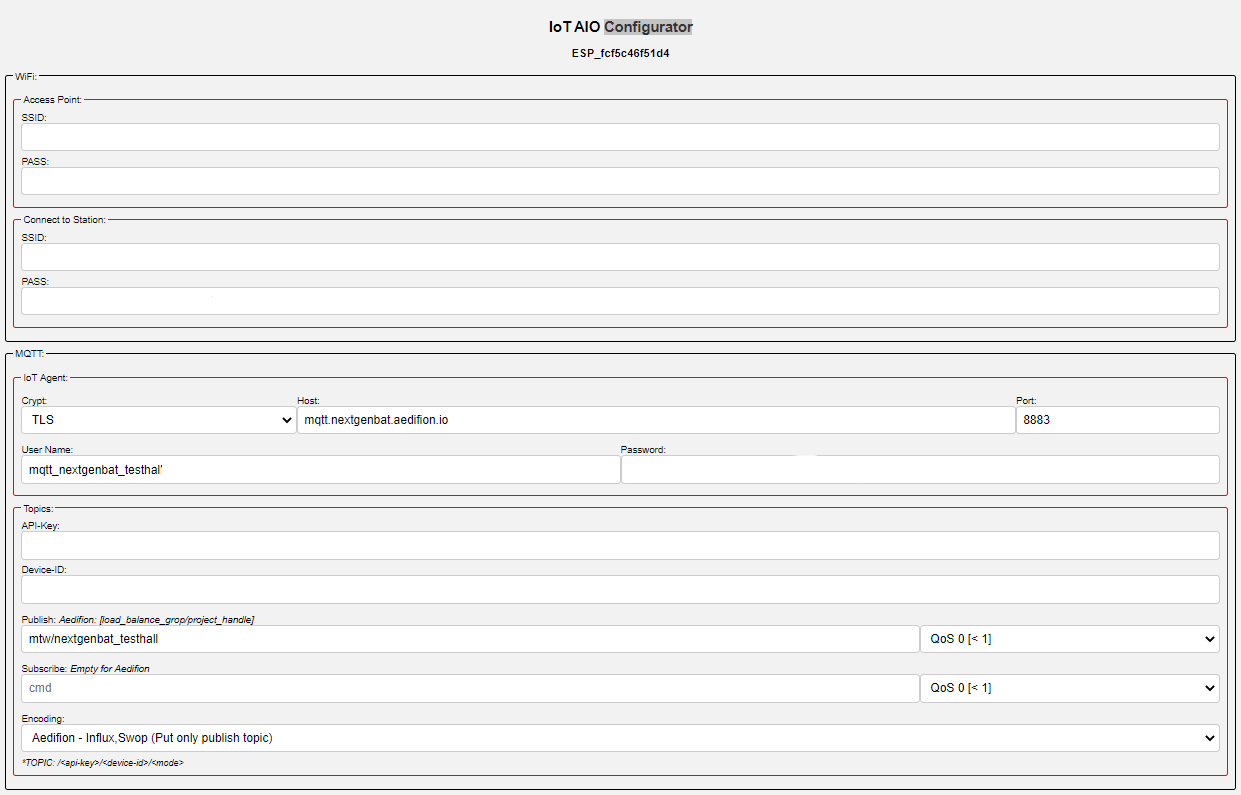
\includegraphics[width=\textwidth]{Figures/configurator.png}
		\caption{IoT Configurator}
		\label{fig:configurator}
	\end{figure}

		\subsection{Wifi}
		The gateway operates as WiFi Access Point or allows connecting to an existing one.
		Both of this can run in parallel.

		\paragraph{Access Point}
		The Access Point mode should only be used for configuration. 
		For example, to save the station credentials on the device.
		The SSID defaults to a device specific name which is composed from ESP and the device's MAC-Address(for example: ESP\_fcf5c46f51d4).
		Hence, every gateway has it's own unique name to distinguish the devices from each other. 
		The password is by default: 123456789

		\paragraph{Station}
		If credentials are entered here, the gateway will try to connect to this Access Point.
\newpage
		\subsection{MQTT}
		The Device will communicate with a cloud server using the MQTT protocol (https://github.com/mqtt/mqtt.github.io/wiki).

		This manual will focus on the connection to the Aedifion (https://www.aedifion.com/) Cloud-platform. However, the gateways also support different MQTT brokers.

		% \paragraph{IoT Agent}
		\paragraph{Topics}
		For connection with Aedifion, the API-Key and Device-ID boxes are not used. Changes to the QoS(Quality of Service) will have no affect on the device's behavior either. \\
		The Publish topic requires only the main Aedifion topic name: For example: `mtw/nextgenbat\_testhall`.
		The following topics will be automatically generated by the device:
			\begin{itemize}
				\item META/mtw/nextgenbat\_testhall
				\item CONTROLS/mtw/nextgenbat\_testhall
				\item mtw/nextgenbat\_testhall/update
			\end{itemize}

		The Aedifion encoding will send the values through the InfluxDB protocol (see \autoref{fig:influx}).\\(https://docs.influxdata.com/influxdb/v1.8/write\_protocols/line\_protocol\_tutorial/)\\
		\begin{figure}[ht!]
		\begin{lstlisting}[language=json,firstnumber=1]
	Datapointname value=20.0 1465839830100400200
				
		\end{lstlisting}
		\caption{Influx message: datapoint, observation, timestamp}
		\label{fig:influx}
		\end{figure}

		The device will receive SWOP(https://aedifion.gitlab.io/swop/) messages on the CONTROLS/... Topic (see \autoref{fig:SWOP}). \\

		\begin{figure}[ht!]
		\begin{lstlisting}[language=json,firstnumber=1]		
{
	"type": 	"NEWSPT",
	"swop-version":	0.1,
	"datapoint": 	"bacnet93-4120-External-Room-Set-Temperature-RTs",
	"value": 	20.3,
	"priority": 	13
}
				\end{lstlisting}
				\caption{SWOP message}
				\label{fig:SWOP}
		\end{figure}
		If the name of a data point matches the name of the SWOP message, the gateway will set the connected device to the given value.

		On each Startup of the gateway, the Metadata will be send to the META/... topic. (see \autoref{fig:Meta})

		\begin{figure}[ht!]
		\begin{lstlisting}[language=json,firstnumber=1]
{
	"name": 	"Name of device",
	"IP": 		"192.168.xxx.xxx",  
	"source": 	"Analog Gateway"
}
		\end{lstlisting}
		\caption{META tag}
		\label{fig:Meta}
		\end{figure}

		\subsection{Data point names}
		For data point naming, we use BUDO (https://github.com/RWTH-EBC/BUDO). BUDO is intended to provide META data in a hierarchical structure allowing artificial-intelligence-based algorithms to identify interrelated devices and topologies.
		The Gateway will automatically parse the unit and send it together with the META-Tags to the Aedifion server. 
		Other names or device keys are applicable as well.

		\subsection{Periodic or Threshold}
		The gateway can publish recorded values periodically or using change of value (COV) (compare \autoref{fig:a-configurator}). 
		% If both inputs are set to periodic, the sampling rate is set to the value of the first input.
		If COV is used the device will check every second the values. 
		If the deviation of one value exceeds the threshold,  all values of the gateway will be published to the MQTT server. 
		In periodic mode the unit is millisecond. 
		In threshold mode, the values are absolute values.

\newpage
	\section{Analog Gateway configuration}
	\begin{figure}[ht!]
		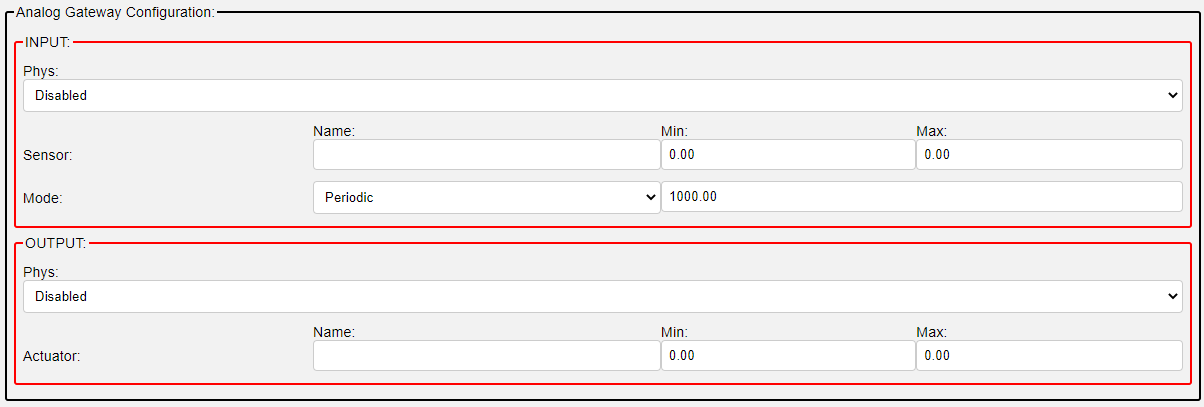
\includegraphics[width=\textwidth]{Figures/5-analog.png}
		\caption{Analog configurator}
		\label{fig:a-configurator}
	\end{figure}
	For the analog gateway, data point names and a user-defined scaling are configured in the Analog Gateway Configuration section.\\
	The analog gateway supports the following interfaces:
	\begin{itemize}
		\item 0(2) - 10 V
		\item 0(4) - 20 mA
	\end{itemize}

	The gateway will scale the input and output according to the user-defined values for minimum and maximum. For example, a 2-10 V signal with a 0-100 \% scaling will map 0 \% to 2 V and 100 \% to 10 V and values within this range accordingly.


% \newpage
	\section{Temperature Gateway configuration}
	\begin{figure}[ht!]
		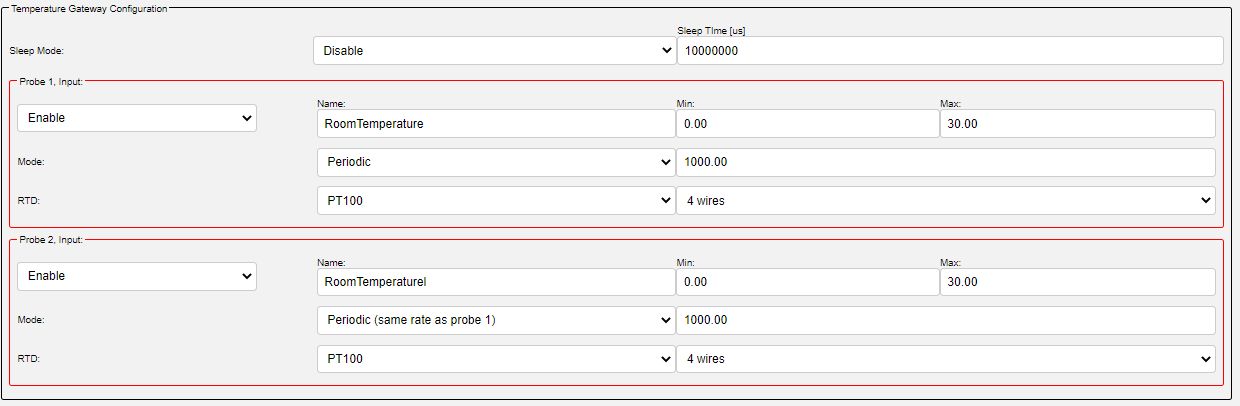
\includegraphics[width=\textwidth]{Figures/3-temp.png}
		\caption{Temperature configurator}
		\label{fig:t-configurator}
	\end{figure}

	For the temperature gateway, data point names, the operational limits and the type of the rtd probe are configured in the Temperature Gateway configuration section. \\

	If the measured value is not within the min and max values, no new value is sent to the cloud server. This is used to protect the device from sending values outside of the operational limits.\\
	
	To achieve the longest possible battery life, it is necessary to set Sleep Mode to enable and use the threshold mode. \\


\newpage
	\section{Digital Gateway configuration}
	\begin{figure}[ht!]
		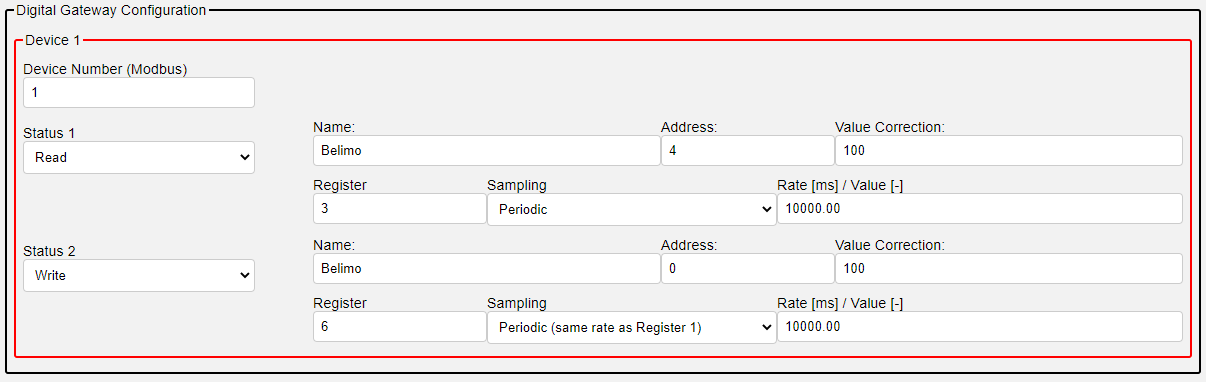
\includegraphics[width=\textwidth]{Figures/2-digital.png}
		\caption{Digital configurator}
		\label{fig:d-configurator}
	\end{figure}
	For the digital gateway, data point names, a user-defined scaling and the connected Modbus device are configured in the Digital Gateway Configuration section. \\

	This configuration is limited to one device and two registers. This limit is only given by the configuration interface. The implemented Modbus stack will support multiple devices and registers.\\


	The Device Number is the Modbus device number. This can be found in the manual of the connected device or can be set manually.
	The name box declares the data point name. This is used for the communication with the Aedifion server.\\

	Each Modbus register can be set up with a read or write command. The function code relates to the register type (input, holding, coil, discrete input; for reference see the Modbus documentation) and should be defined in the Register box. The correct values can be found in the manual of the field device. In the address field, the corresponding register address has to be entered which is usually given by the vendor in the data sheet of the field device.\\

	To adjust the output value, the correction box needs to be filled.
	The real value from the field device is then divided by the given value in the input box. \\
	For example:\\
	The Belimo Modbus devices store their set points in a value between 0 and 10000. If a 0 to 100 \% representation is desired, the incomming signal has to be divided by factor 100. 



\end{document}